\documentclass[14pt, a4paper]{extarticle}
\usepackage{GOST}
\usepackage{array}
\usepackage{verbatim}
\usepackage[detect-all]{siunitx}
\usepackage{amsmath}
\usepackage{amssymb}
\usepackage[utf8]{inputenc}
\usepackage{hyperref}
\usepackage{tempora}

\makeatletter
\renewcommand\@biblabel[1]{#1.}
\makeatother

\usepackage{listings}
\lstset{ 
	language=python,
	basicstyle=\small\sffamily, 
	numbers=left, 
	numberstyle=\tiny,
	stepnumber=1,
	numbersep=5pt,
	showspaces=false,            
	showstringspaces=false,      
	showtabs=false,             
	frame=single,            % рисовать рамку вокруг кода
	tabsize=4,      
	commentstyle=\color{green},
	keywordstyle=\color{blue}\textbf,
	numberstyle=\scriptsize\color{gray}, % the style that is used for the line-numbers
	rulecolor=\color{black},
	captionpos=t,
	breaklines=true,         % автоматически переносить строки 
	breakatwhitespace=false, % переносить строки по пробелу
	escapeinside={\#*}{*)} 
}


\usepackage{pgfplots}
\usepackage{filecontents}
\usetikzlibrary{datavisualization}
\usetikzlibrary{datavisualization.formats.functions}

\begin{document}
	
\begin{table}[ht]
	\centering
	\begin{tabular}{|c|p{400pt}|} 
		\hline
		\begin{tabular}[c]{@{}c@{}} 
\includegraphics[scale=1]{source/b_logo.jpg} \\\end{tabular} &
		\footnotesize\begin{tabular}[c]{@{}c@{}}\textbf{Министерство~науки~и~высшего~образования~Российской~Федерации}\\\textbf{Федеральное~государственное~бюджетное~образовательное~учреждение}\\\textbf{~высшего~образования}\\\textbf{«Московский~государственный~технический~университет}\\\textbf{имени~Н.Э.~Баумана}\\\textbf{(национальный~исследовательский~университет)»}\\\textbf{(МГТУ~им.~Н.Э.~Баумана)}\\\end{tabular}  \\
		\hline
	\end{tabular}
\end{table}
\noindent\rule{\textwidth}{4pt}
\noindent\rule[14pt]{\textwidth}{1pt}
\hfill 
\noindent
\makebox{ФАКУЛЬТЕТ~}%
\makebox[\textwidth][l]{\underline{~«Информатика и системы управления»~~~~~~~~~~~~~~~~~~~~~~~~~~~~~~~~~}}%
\\
\noindent
\makebox{КАФЕДРА~}%
\makebox[\textwidth][l]{\underline{~«Программное обеспечение ЭВМ и информационные технологии»~}}%
\\

\begin{center}
	\vspace{1.5cm}
	{\bf\huge Отчёт\par}
	{\bf\Large по лабораторной работе № 4\par}
	\vspace{0.7cm}
\end{center}


\noindent
\makebox{\large{\bf Название:}~~~}
\makebox[\textwidth][l]{\large\underline{~Параллельное умножение матриц~}}\\

\noindent
\makebox{\large{\bf Дисциплина:}~~~}
\makebox[\textwidth][l]{\large\underline{~Анализ алгоритмов~~~~~~~~~~~~~~~~~~~~~~~~~~}}\\

\vspace{1.5cm}
\noindent
\begin{tabular}{l c c c c c}
	Студент      & ~ИУ7-55Б~               & \hspace{2.5cm} & \hspace{2cm}                 & &  Д.О. Склифасовский \\\cline{2-2}\cline{4-4} \cline{6-6} 
	\hspace{3cm} & {\footnotesize(Группа)} &                & {\footnotesize(Подпись, дата)} & & {\footnotesize(И.О. Фамилия)}
\end{tabular}

\noindent
\begin{tabular}{l c c c c}
	Преподователь & \hspace{5cm}   & \hspace{2cm}                 & & ~~~~~~Л.Л. Волкова~~~~~~\\\cline{3-3} \cline{5-5} 
	\hspace{3cm}  &                & {\footnotesize(Подпись, дата)} & & {\footnotesize(И.О. Фамилия)}
\end{tabular}

\vspace{0.6cm}
\begin{center}	
	\vfill
	\large \textit {Москва, 2020}
\end{center}

\thispagestyle {empty}
\pagebreak

% СОДЕРЖАНИЕ 
\clearpage
\tableofcontents

% ВВЕДЕНИЕ
\clearpage
\section*{Введение}
\addcontentsline{toc}{section}{Введение}
Цель работы: изучение возможности параллельных вычислений и использование такого подхода на практике.\par
В ходе лабораторной работы требуется:
\begin{enumerate}
	\item[1)] выбрать алгоритм для рассмотрения;
	\item[2)] описать обычную версию;
	\item[3)] выполнить 2 параллельные версии;
	\item[4)] запустить эксперименты на каждый при различном числе потоков 1,2,4,8 ...4M, где M - количество логических ядер на компьютере;
	\item[5)] проверить, всегда ли при росте потоков, время работы снижается;
	\item[6)] описать главный и рабочий поток схемой;
	\item[7)] описать точки сборки.
\end{enumerate}
В данной лабораторной работе был выбран алгоритм Винограда. Необходимо сравнить зависимость времени работы алгоритма от числа параллельных потоков и размера матриц, провести сравнение стандартного и параллельного алгоритмов.

% АНАЛИТИЧЕСКИЙ РАЗДЕЛ
\clearpage
\section{Аналитический раздел}
В данном разделе представлено описание стандартного и параллельного алгоритмов Винограда.
\subsection{Общие сведения}
Матрица — математический объект, записываемый в виде прямоугольной таблицы элементов кольца или поля (например, целых, действительных или комплексных чисел), которая представляет собой совокупность строк и столбцов, на пересечении которых находятся её элементы. Количество строк и столбцов задает размер матрицы. Хотя исторически рассматривались, например, треугольные матрицы, в настоящее время говорят исключительно о матрицах прямоугольной формы, так как они являются наиболее удобными и общими. \par
Умножение матриц — одна из основных операций над матрицами. Матрица, получаемая в результате операции умножения, называется произведением матриц.
\subsection{Алгоритм Винограда}
Если посмотреть на результат умножения двух матриц, то видно, что каждый элемент в нем представляет собой скалярное произведение соответствующих строки и столбца исходных матриц. Можно заметить также, что такое умножение допускает предварительную обработку, позволяющую часть работы выполнить заранее. \hyperref[literature]{[1]}\par
Рассмотрим два вектора $V = (v_{1},v_{2},v_{3},v_{4})$ и $W = (w_{1},w_{2},w_{3},w_{4})$. Их скалярное произведение равно:
\begin{equation}
	V * W = v_{1}w_{1} + v_{2}w_{2} + v_{3}w_{3} + v_{4}w_{4}
\end{equation}
Это равенство можно переписать в виде:
\begin{equation}
	V * W = (v_{1} + w_{2})(v_{2} + w_{1}) + (v_{3} + w_{4})(v_{4} + w_{3}) -  v_{1}v_{2} - v_{3}v_{4} - w_{1}w_{2} - w_{3}w_{4}
\end{equation}
Менее очевидно, что выражение в правой части последнего равенства допускает предварительную обработку: его части можно вычислить заранее и запомнить для каждой строки первой матрицы и для каждого столбца второй. На практике это означает, что над предварительно обработанными элементами придется выполнять лишь первые два умножения и последующие пять сложений, а также дополнительно два сложения. 
\subsection{Параллельное программирование}
Параллельное программирование. Параллельное программирование служит для создания программ, эффективно использующих вычислительные ресурсы за счет одновременного исполнения кода на нескольких вычислительных узлах. Для создания параллельных приложений используются параллельные языки программирования и специализированные системы поддержки параллельного программирования, такие как MPI и OpenMP. Параллельное программирование является более сложным по сравнению с последовательным как в написании кода, так и в его отладки. Для облегчения процесса параллельного программирования существуют специализированные инструменты, например, отладчик TotalView.\hyperref[literature]{[2]}
\subsection{Параллельный алгоритм Винограда}
Для того, чтобы добиться большей эффективности алгоритма умножения матриц Винограда, необходимо расспараллелить ту часть алгоритма, которая содержит больше всего вложенных циклов. Вычисление результата для каждой строки не зависит от результата умножения для других строк. Каждый поток будет выполнять вычисления определенных строк результирующей матрицы.\par
Для проверки эффективности выбранного метода, также можно распараллелить циклы двойной вложенности в начале алгоритма (циклы вычисления векторов mulH и mulV).
\subsection{Вывод}
Было представлено математическое описание стандартного и параллельного алгоритмов Винограда. Основная идея заключается в том, чтобы распараллелить главный цикл тройной вложенности.

\clearpage
\section{Конструкторский раздел}
В данном разделе представлены схемы разработанных алгоритмов. Также описывается часть алгоритма, которая будет распараллеливаться.
\subsection{Разработка алгоритма}
На \hyperref[Algorithm1]{рисунке 1} изображена схема стандартного алгоритма умножения матриц.
\begin{figure}[h!]\label{Algorithm1}
	\center{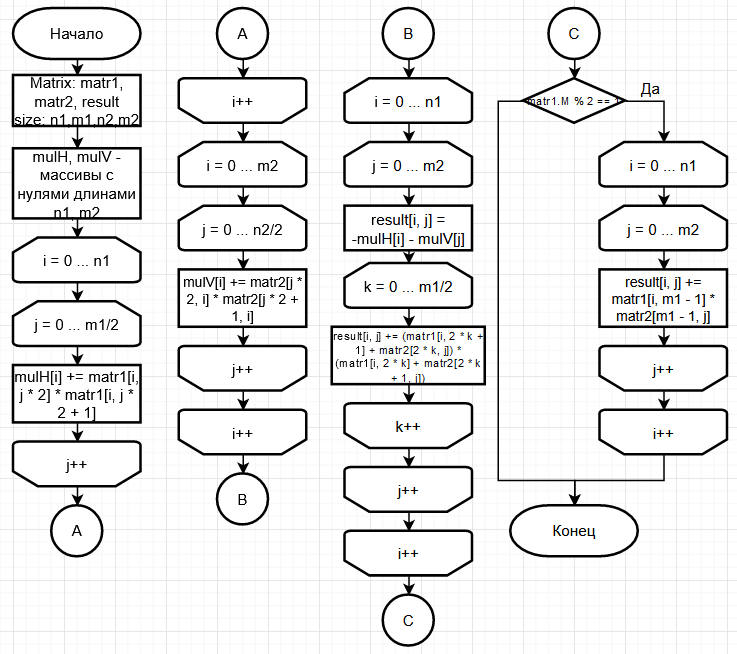
\includegraphics[scale=1.1]{source/Algorithm.png}}
	\caption{Схема стандартного алгоритма умножения матриц}
\end{figure}
\subsection{Распараллеливание программы}
В представленном алгоритме будет распараллеливаться цикл тройной вложенности (участок между B и C). Это должно ускорить время работы алгоритма.\par
Также для проверки эффективности будут распараллеливаться два первых цикла отдельно. Будут построены графики для данной реализации и сравниться время работы алгоритмов.
\subsection{Вывод}
В данном разделе была рассмотрена схема алгоритма Винограда и описалась часть алгоритма, которая будет распараллеливаться.

\clearpage
\section{Технологический раздел}
В данном разделе даны общие требования к программе, средства реализации и сама реализация алгоритмов.
\subsection{Общие требования}
\textbf{Требования к вводу:}
\begin{enumerate}
	\item[1)] вводятся размеры матриц;
	\item[2)] вводятся (или автоматически генерируются) матрицы. 
\end{enumerate}\par
\textbf{Требования к программе}
\begin{enumerate}
	\item[1)] при вводе неправильных размеров матриц программа не должна завершиться аварийно;
	\item[2)] должно выполняться корректное умножение матриц.
\end{enumerate}
\subsection{Средства реализации}
В качестве языка программирования был выбран C\#, так как я знаком с данным языком программирования, имею представление о способах тестирования программы.\hyperref[literature]{[3]}\par
Средой разработки Visual Studio.\hyperref[literature]{[4]}\par 
Для замеров процессорного времени используется функция $Stopwatch$.\hyperref[literature]{[5]}\hyperref[literature]{[6]}\par
Многопоточное программирование было реализовано с помощью пространства имен System.Threading.\hyperref[literature]{[7]}
\subsection{Сведения о модулях программы}
Программа состоит из:
\begin{enumerate}
	\item[1)] Program.cs - главный файл программы, в котором располагается точка входа в программу;
	\item[2)] Matrix.cs - файл класса Matrix. Класс реализует матрицу размером $n * m$, а также он содержит методы для работы с матрицами;
	\item[3)] Parameters.cs - файл классов ParametersForFirst и ParametersForSecond, которые используются для передачи данных функциям при распараллеливании циклов;
	\item[4)] MultMatr.cs - файл класса MultMatr. В нем находится алгоритм Винограда;
	\item[5)] ParallelMultMatr.cs - файл класса ParallelMultMatr, в котором находятся параллельныи реализации алгоритма Винограда.
\end{enumerate}
\subsection{Листинг кода программы}
В листинге 1 реализован стандартный алгоритм Винограда.
\begin{lstlisting}[label=MultMatrVin, caption=Стандартный алгоритм Винограда]
	public static Matrix VinogradMult(Matrix matr1, Matrix matr2)
	{
		int n1 = matr1.N;
		int n2 = matr2.N;
		int m1 = matr1.M;
		int m2 = matr2.M;
		if ((m1 != n2) || n1 == 0 || n2 == 0)
		{
			return null;
		}
		
		Matrix result = new Matrix(n1, m2);
		int[] mulH = new int[n1];
		int[] mulV = new int[m2];
		
		for (int i = 0; i < n1; i++)
		{
			for (int j = 0; j < m1 / 2; j++)
			{
				mulH[i] += matr1[i, j * 2] * matr1[i, j * 2 + 1];
			}
		}
		
		for (int i = 0; i < m2; i++)
		{
			for (int j = 0; j < n2 / 2; j++)
			{
				mulV[i] += matr2[j * 2, i] * matr2[j * 2 + 1, i];
			}
		}
		
		for (int i = 0; i < n1; i++)
		{
			for (int j = 0; j < m2; j++)
			{
				result[i, j] = -mulH[i] - mulV[j];
				for (int k = 0; k < m1 / 2; k++)
				{
					result[i, j] += (matr1[i, 2 * k + 1] + matr2[2 * k, j]) * (matr1[i, 2 * k] + matr2[2 * k + 1, j]);
				}
			}
		}
		
		if (m1 % 2 == 1)
		{
			for (int i = 0; i < n1; i++)
			{
				for (int j = 0; j < m2; j++)
				{
					result[i, j] += matr1[i, m1 - 1] * matr2[m1 - 1, j];
				}
			}
		}
		
		return result;
	}
\end{lstlisting}
В листинге 2 реализован параллельный алгоритм Винограда
\begin{lstlisting}[label=ParallelMulVin, caption=Параллельный алгоритм Винограда]
	public static Matrix ParallelVinogradMult1(Matrix matr1, Matrix matr2, int countOfThreads)
	{
		int n1 = matr1.N;
		int n2 = matr2.N;
		int m1 = matr1.M;
		int m2 = matr2.M;
		if ((m1 != n2) || n1 == 0 || n2 == 0)
		{
			return null;
		}
		
		Matrix result = new Matrix(n1, m2);
		int[] mulH = new int[n1];
		int[] mulV = new int[m2];
		
		for (int i = 0; i < n1; i++)
		{
			for (int j = 0; j < m1 / 2; j++)
			{
				mulH[i] += matr1[i, j * 2] * matr1[i, j * 2 + 1];
			}
		}
		
		for (int i = 0; i < m2; i++)
		{
			for (int j = 0; j < n2 / 2; j++)
			{
				mulV[i] += matr2[j * 2, i] * matr2[j * 2 + 1, i];
			}
		}
		
		Thread[] threads = new Thread[countOfThreads];
		int distribution = n1 / countOfThreads;
		int startI = 0;
		for (int i = 0; i < countOfThreads; i++)
		{
			int endI = startI + distribution;
			if (i == countOfThreads - 1)
			{
				endI = n1;
			}
			ParametersForFirst param = new ParametersForFirst(result, matr1, matr2, mulV, mulH, startI, endI, m2, m1);
			threads[i] = new Thread(ComputationLoopForMain);
			threads[i].Start(param);
			startI = endI;
		}
		foreach (Thread curThread in threads)
		{
			curThread.Join();
		}
		
		if (m1 % 2 == 1)
		{
			for (int i = 0; i < n1; i++)
			{
				for (int j = 0; j < m2; j++)
				{
					result[i, j] += matr1[i, m1 - 1] * matr2[m1 - 1, j];
				}
			}
		}
		
		return result;
	}
\end{lstlisting}
В листинге 3 реализован алгоритм Винограда с распараллеленым алгритмом Винограда
\begin{lstlisting}[label=loop, caption=Распараллеленный главный цикл]
	private static void ComputationLoopForMain (object curObj)
	{
		ParametersForFirst param = (ParametersForFirst)curObj;
		int startI  = param.startI, 
			endI    = param.endI,
			m2      = param.m2, 
			m1      = param.m1;
		Matrix res  = param.res,
			matr1   = param.matr1,
			matr2   = param.matr2;
		int[] mulH  = param.mulH,
			mulV    = param.mulV;
		
		for (int i = startI; i < endI; i++)
		{
			for (int j = 0; j < m2; j++)
			{
				res[i, j] = -mulH[i] - mulV[j];
				for (int k = 0; k < m1 / 2; k++)
				{
					res[i, j] += (matr1[i, 2 * k + 1] + matr2[2 * k, j]) * (matr1[i, 2 * k] + matr2[2 * k + 1, j]);
				}
			}
		}
	}
\end{lstlisting}
\subsection{Вывод}
В данном разделе были даны общие требования к программе, описаны средства реализации, были представлены сведения о модулях программы, а также реализованы алгоритмы умножения матриц (Винограда и параллельный Винограда).

\clearpage
\section{Экспериментальный раздел}
В данном разделе представлены результаты работы программы и приведен анализ времени работы алгоритмов.
\subsection{Описание экспериментов}
Было произведено 2 серии замеров:
\begin{enumerate}
	\item[1)] для матриц размером $N x N = 300$ при переменном числе потоков для параллельных реализаций;
	\item[2)] для матриц размером $N x N, N \in \{100,200,300,400,500,600,700\}$ с постоянным числом потоков для параллельных реализаций.
\end{enumerate}
\subsection{Технические характеристики устройства, на котором проводились замеры}
\begin{enumerate}
	\item[1)] операционная система Windows 10 64-bit;
	\item[2)] память 8 ГБ;
	\item[3)] процессор AMD Ryzen 5 3500U CPU @ 2.1GHz;
	\item[4)] 8 логических процессоров.
\end{enumerate}
\clearpage
\subsection{Примеры работы программы}
На \hyperref[Example1]{рисунке 2} представлен результат работы алгоритмов.
\begin{figure}[h!]
	\centering
	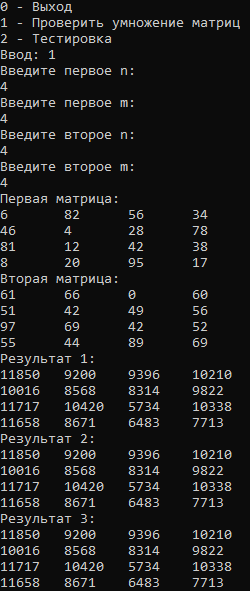
\includegraphics[scale=1]{source/Example1.png}
	\caption{Первый результат работы программы}
	\label{Example1}
\end{figure}\par
\clearpage
На \hyperref[Example2]{рисунке 3} представлен второй результат работы алгоритмов.
\begin{figure}[h!]
	\centering
	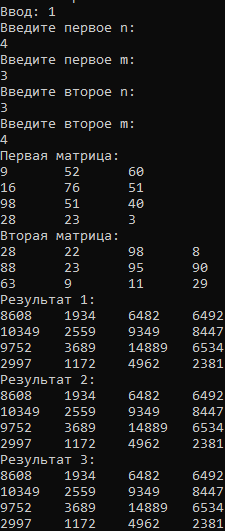
\includegraphics[scale=1]{source/Example2.png}
	\caption{Второй результат работы программы}
	\label{Example2}
\end{figure}\par
\clearpage
\subsection{Анализ времени работы алгоритмов}
На \hyperref[Test1]{рисунке 4} представлен график зависимости времени работы алгоритмов и количества потоков.\par
Для передачи в распараллеленную функцию данных в C\# необходимо передавать данные только в объекте, изначально создается объект, который хранит необходимые данные, и в функцие данные переприсваиваются переменным. Из-за этого время работы 2 параллельной реализации будет намного больше линейной реализации и 1 параллельной реализации.
\begin{figure}[h!]
	\centering
	\begin{tikzpicture}[object/.style={thin,double,<->}]
		
		\begin{axis}[
			axis lines = left,
			xlabel = $\textit{количество потоков в параллельных реализациях}$,
			ylabel = {$\textit{время выполнения, тики}$},
			legend pos=north east,
			ymajorgrids=true
			]
			\addplot[color=red] table[x index=0, y index=1] {source/FirstExp1.dat}; 
			\addplot[color=orange] table[x index=0, y index=1] {source/FirstExp2.dat};
			\addplot[color=blue, mark=square] table[x index=0, y index=1] {source/FirstExp3.dat};
			
			\addlegendentry{Линейная реализация}
			\addlegendentry{Параллельная реализация 1}
			\addlegendentry{Параллельная реализация 2}
			
		\end{axis}
	\end{tikzpicture}
	
	\caption{Результаты замеров процессорного времени в первом эксперименте.}
	\label{Test1}
\end{figure}
\clearpage
На \hyperref[Test2]{рисунке 5} представлен график зависимости времени работы алгоритмов и размера матриц.\par
Из-за того, что замеры проводятся с 8 логическими процессорами - эффективнее всего использовать 8 потоков.
\begin{figure}[h!]
	\centering
	\begin{tikzpicture}[object/.style={thin,double,<->}]
		
		\begin{axis}[
			axis lines = left,
			xlabel = $\textit{размер матриц}$,
			ylabel = {$\textit{время выполнения, тики}$},
			legend pos=north east,
			ymajorgrids=true
			]
			\addplot[color=red] table[x index=0, y index=1] {source/SecondExp1.dat}; 
			\addplot[color=orange] table[x index=0, y index=1] {source/SecondExp2.dat};
			\addplot[color=blue, mark=square] table[x index=0, y index=1] {source/SecondExp3.dat};
			
			\addlegendentry{Линейная реализация}
			\addlegendentry{Параллельная реализация 1}
			\addlegendentry{Параллельная реализация 2}
			
		\end{axis}
	\end{tikzpicture}
	
	\caption{Результаты замеров процессорного времени во втором эксперименте.}
	\label{Test2}
\end{figure}
\clearpage
\subsection{Вывод}
Результаты тестирования показывают, что, во-первых, с увеличением количества потоков увеличивается время работы параллельной реализации 2. Линенйая реализация показывает одинаковый результат. А параллельная реализация 2 показывает, что при 8 потоках - она наиболее эффективна, а с увеличением увеличивается время.\par
Во-вторых, при одинаковом количестве потоков и разных размерах матриц, самым эффективной является вторая параллельная реализация, а первая и линейная работают идентично.\par
Можно сделать вывод, что самой эффективной реализацией является вторая и, что следует распараллеливать главный цикл (состоящий из 3 вложенных циклов).

\clearpage
\section{Заключение}
В ходе выполнения лабораторной работы были изучены возможности параллельных вычислений и был использован такой подход на практике. Были даны теоритически оценки алгоритмов умножения матриц. Также сравнили время работы алгоритмов, в результате которого стало понятно, что самой эффективной реализацией была та, когда было необходимо распараллелить главный цикл алгоритма Винограда. Данная реализация быстрее линейной примерно в 2.5 раза.


\clearpage
\section*{Литература}
\addcontentsline{toc}{section}{Литература}
\begin{enumerate}
	\label{literature}
	\item Умножение матриц. -URL: \href{http://www.algolib.narod.ru/Math/Matrix.html}{http://www.algolib.narod.ru/Math/Matrix.html} (дата обращения: 24.10.2020). -Текст: электронный.
	\item Параллельное программирование. -URL: \href{https://www.viva64.com/ru/t/0038/}{https://www.viva64.com/ru/t/0038/} (дата обращения: 24.10.2020). -Текст: электронный.
	\item  Документация по C\#. -URL: \href{https://docs.microsoft.com/ru-ru/dotnet/csharp/}{https://docs.microsoft.com/ru-ru/dotnet/csharp/} (дата обращения: 24.10.2020). -Текст: электронный.
	\item Документация по семейству продуктов Visual Studio. -URL:\par \href{https://docs.microsoft.com/ru-ru/visualstudio/?view=vs-2019}{https://docs.microsoft.com/ru-ru/visualstudio/?view=vs-2019 } (дата обращения: 01.10.2020). -Текст: электронный.
	\item Stopwatch Класс. -URL: \href{https://goo.su/2e99}{https://goo.su/2e99 } (дата обращения: 24.10.2020). -Текст: электронный.
	\item Под капотом у Stopwatch. -URL:  \href{https://habr.com/ru/post/226279/}{https://habr.com/ru/post/226279/} (дата обращения: 24.10.2020). Текст: электронный.
	\item Thread Класс. -URL: \href{https://docs.microsoft.com/ru-ru/dotnet/api/system.threading.thread?view=netcore-3.1}{https://docs.microsoft.com/ru-ru/dotnet/api/system.threading.thread?view=netcore-3.1} (дата обращения 24.10.2020). -Текст: электронный.
\end{enumerate}
\end{document}\par